\title{Estándares de Usabilidad UI}

\author{\IEEEauthorblockN{Abraham Jhared Flores Azcona}
\IEEEauthorblockA{\textit{Depto. De Sistemas y Computación} \\
\textit{Instituto Tecnológico de Tijuana}\\
Tijuana, Baja California, México \\
abraham.flores193@tectijuana.edu.mx}
}

\maketitle

\begin{abstract}
El diseño de una UI envuelve distintos ámbitos de múltiples dominios del conocimiento
que le permite considerar distintas perspectivas para entregar productos relevantes, sin embargo
debido a la abundancia de la información, la disciplina de diseño de UI se ve obligada a optar
por ciertos lineamientos que guíen el proceso. En la presente investigación se explican 
los estándares de calidad para las intefaces de usuario así como el análisis de los 
estándares de calidad que aplican a la plataforma web de \emph{reddit}.
\end{abstract}

\section{Introducción}
El diseño de interfaces de usuario consiste generalmente en la realización del aspecto
visual de una aplicación \cite{tutorialspoint-2021,geeksforgeeks-2022,unknown-author-no-dateA},
mientras que la literatura académica \cite{sharma-2021} complementa la definición
al incluír la interacción entre el dispositivo y el usuario por medio de técnicas 
ó comandos para operar el dispositivo, introducir datos, y usar los contenidos provistos
donde la forma concreta de evaluar dichos aspectos se conoce como Usabilidad.
Como cualquier disciplina, se necesita la disponibilidad de recursos que indiquen exactamente
que aspectos considerar para el diseño de la Usabilidad de UI porque cada persona puede argumentar la razón
por la que su propuesta sea la mejor; esto se puede contrarestar con el desarrollo, implementación
y adoptación de estándares de calidad para tener una formalidad y consistencia de producto y producción
del mismo . % TODO citar a Bevan

\section{Estándares de Calidad}
Para poder aplicar los estandares de usabilidad existenes, es sumamente importante conocer la
definición concreta respecto a qué son los Estándares de Calidad. Para % TODO citar a safetyculture, ASQ y NIBUSINESS
nos referimos a conjuntos de lineamientos, sistemas, métodos, requerimientos y especificaciones
seguidas por una organización para asegurar un proceso consistente y una calidad de productos.
% TODO citar ASQ
agrega que dichos estándares le proveen a distintas organizaciones una visión , entendimiento,
procesos y vocabulario mútuos que son necesarios para alcanzar las expectativas de los involuctrados.
mutuo.
\begin{figure}[t]
    \centering
    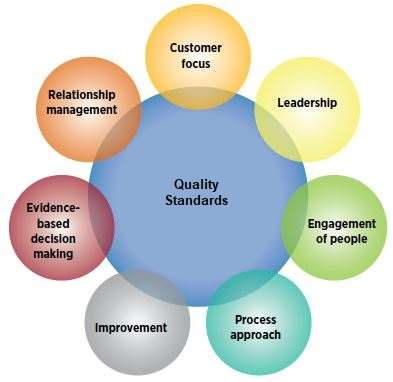
\includegraphics[scale=0.5]{../images/fig1.JPG}
    \caption{Principios fundamentales de los Estándares de Calidad.}
    \label{fig:fig1}    
\end{figure}

\subsection{Institución más reconocida: ISO}
La institución más reconocida y reputable en los estándares de calidad es aquella de la ISO
(La Organización Internacional de Estándares por sus siglas en inglés) que es una organización
no gubernamental que se forma en gran parte por una red globale de cuerpos de estandarización
donde su principal finalidad es la creación de estándares donde la ISO provee una plataforma
para desarrollar herramientas por medio de la cooperación y el entendimiento mútuo. % TODO citar al ISO

\subsubsection{Estándares más populares}
La siguiente lista es tomada de lo expuesto en % TODO citar a Horielikova
que muestra los 12 estándares populares de la ISO en 2019.
\begin{enumerate}
    \item ISO 9001; incluye los sistemas de control de calidad donde generamente la version ISO 9001:2015 es la más utilizada ya menciona los requerimientos. % TODO citar ISO 9001
    \item ISO 14001; la revisión ISO 14001:2015 es la más utilizada y especifica los requerimientos y lineamientos para los sistemas de gestión ambiental. % TODO cite ISO 14001
    \item ISO 45001; su revisión de 2022 es la más reciente y explica los requerimientos y lineamientos para los sistemas gestores de salúd y seguridad ocupacional. % TODO cite ISO 45001
    \item ISO 22000; la versión actual es la de 2018 y éste estandar menciona los requerimientos para cualquier organización de la cadena alimenticia en lo competente a sistemas gestores de seguridad alimenticia. % TODO cite ISO 22000
    \item ISO/IEC 27001; la versión del 2022 explica los requerimientos respecto a los sistemas de gestión de seguridad informática en el ámbito de la seguridad informática, ciberseguridad y protección de privacidad. % TODO cite ISO/IEC 27001
    \item ISO 13485:2003 \& 2016; sus versiones explican los requerimientos para fines regulatorios para sistemas de gestión de calidad para dispositivos médicos. % TODO cite ISO 13485
    \item ISO 50001; aunado a su revisión de 2018, éste explica los requerimientos y lineamientos de uso para sistemas gestores de energía. % TODO citar ISO 50001
    \item ISO/IEC 20000-1; con la revisión de 2018, dicho estándar expone los requerimientos para sistemas gestores de servicios para IT. % TODO citar ISO/IEC 200001-1
    \item ISO 28000; con sus versión de 2022, el estándar especifica los requerimientos para sistemas gestores de seguridad en el área de seguridad y resiliencia. % TODO citar ISO 28000
    \item ISO 22301; su versión más reciente es la del 2019 y expone los requerimientos para sistemas gestores de continuidad de negocios en lo que respecta el área de seguridad y resiliencia. % TODO citar ISO 22301
    \item ISO 37001; con la revisión de 2016 se exponen los requerimientos y lineamientos para sistemas gestores anti-sobornos. % TODO citar ISO 37001
    \item ISO 39001; la versión de 2012 explica los requerimientos y lineamientos para los sistemas gestores de seguridad de tráfico vial. % TODO citar ISO 39001
\end{enumerate}

\section{Usabilidad}
La usabilidad es una medida que de acuerdo a la Fundación de Diseño de Interacción \cite{unknown-author-no-dateC}, % TODO citar a la fundación
permite a un usuario específico utilizar un producto/diseño en un contexto dado para lograr
un objetivo especifico de manera efectiva, eficiente y satisfactoriamente. \cite{unknown-author-no-dateB} menciona % TODO citarlo
que dicha usabilidad es un atributop cualitativo, por lo que tendremos inherentemente una
evaluación sesgada, sin embargo lista cinco elementos que concretan la definición:
(1) Facilidad de aprendizaje, (2) Eficiencia, (3) Facilidad de memorización, (4) Errores 
y (5) Satisfacción.
\\

Otras definiciones, como la de \cite{guntupalli-no-date} % TODO citarlo
incluyen que la usabilidad (en el contexto de las interfaces de usuario),
es compuesta de tres disciplinas del diseño: De interacción, de información y de 
interfaz. El diseño de información destaca bastante debido a no ser frecuentemente mencionado como 
parte del diseño de la usabilidad en distintos articulos y dihco elemento se define como la forma en 
que se muestran los datos que permiten al usuario discernir si son relevantes para la tarea a realizar.
\\

Otras consideraciones importantes que \cite{joo-2017}  % TODO citarla
menciona son aquellas de las areas para el diseño mas apropiado de una UI/UX que consisten en:
(1) El conocimiento básico de UI/UX, (2) Establecer los puntos a investigar para el diseño,
(3) Establecer el concepto unificador de diseño como lo es las palabras clave del producto y
(4) El diseño de la producción, que considera aspectos técnicos tales como la resolución y la tipografía.

\subsection{Estándares de calidad ISO en la Usabilidad de UI}
A pesar de ser un tema extenso, la ISO si nos ofrece una serie de estándares para asegurar
la calidad de la usabilidad en UI. Sin embargo como se menciona en % TODO citar a Bevan
los estandares ISO respecto al tema son muy complicados de utilizar para los diseñadores a pesar
de ser un buen cimiento para el conocimiento de UI y Usabilidad estandarizada. Para esta redacción
funcionan como un primer acercamiento a la estandarización de la Usabilidad UI.
\\

El principal estándar ISO que se puede aplicar a la usabilidad es aqul del ISO 9241-210 % TODO citar ISO 9241-210
que expone el acercamiento del diseño centrado en humanos para sistemas interactivos en el área de
de la ergonomía en la interacción humano-sistema. 

\section{Ejemplo: Reddit}
Reddit es una plataforma que le permite a los usuarios crear foros (llamados \emph{subreddits}) y
publicar, comentar, compartir y votar contenidos provenientes dentro o fuera de la plataforma.
\begin{figure}[t]
    \centering
    
\includegraphics[scale=0.33]{../images/fig2.png}
    \caption{Despliegue de inicio de usuario de reddit.}
    \label{fig:fig2}    
\end{figure}
\\

Es importante destacar que la interfaz a analizar es aquella del \emph{new} reddit (Fig. \ref{fig:fig2}), que es
más familiar con otras páginas web contemporaneas, mientras que su contraparte de \emph{old}
reddit es la versión original del sitio, que se caracteríza por ser muy parecida a las paginas
web de los 90s.
\\

Respecto a los estandares de calidad que se pueden encontrar para la aplicación, el único documento pertinente
que explica de la manera más comprensiva posible son los Lineamientos de Comarca de Reddit % TODO citar Reddit
provistos en la página oficial de la aplicación; debido a ello, se refiere en lo subsecuente de la investigación
al reporte de los lineamientos internos de Reddit para inferir posibles estándares de usabilidad ISO.

\subsection{Lineamientos Internos}

\subsection{Estandares ISO aplicables}

\section{Conclusión}

\bibliographystyle{IEEEtran}
\bibliography{bibliography}